%label:"fig:LefschetzFibrationForCotangentBundleOfASphere"
%type:"figure"
%name:" Lefschetz fibration for cotangent bundle of a sphere"
%caption:"Lefschetz fibration for the cotangent bundle of the sphere"
%parent:""

        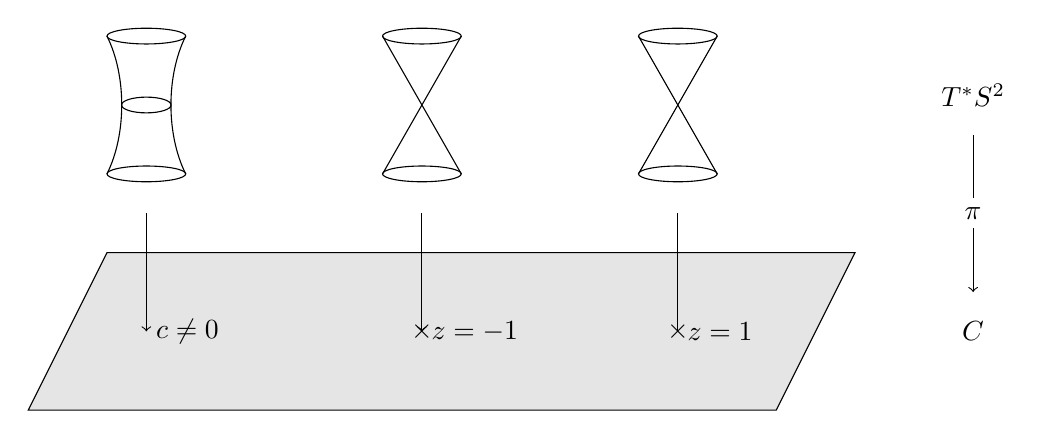
\begin{tikzpicture}

\draw[fill=gray!20] (-2.5,2.5) -- (-3.5,0.5) -- (6,0.5) -- (7,2.5) -- cycle;
\begin{scope}[scale=0.5, shift={(7,3.5)}]
\draw  (-4,7) ellipse (1 and 0.2);
\draw  (-4,3.5) ellipse (1 and 0.2);
\draw (-5,7) -- (-3,3.5) (-5,3.5) -- (-3,7);
\end{scope}
\begin{scope}[scale=0.5, shift={(13.5,3.5)}]
\draw  (-4,7) ellipse (1 and 0.2);
\draw  (-4,3.5) ellipse (1 and 0.2);
\draw (-5,7) -- (-3,3.5) (-5,3.5) -- (-3,7);
\end{scope}
\begin{scope}[scale=0.5,shift={(0,3.5)}]
\draw  (-4,7) ellipse (1 and 0.2);
\draw  (-4,3.5) ellipse (1 and 0.2);

\draw (-5,7) .. controls (-4.5,6) and (-4.5,4.5) .. (-5,3.5);
\draw (-3,7) .. controls (-3.5,6) and (-3.5,4.5) .. (-3,3.5);
\draw  (-4,5.25) ellipse (0.63 and 0.2);
\end{scope}

\draw[->] (-2,3) -- (-2,1.5);
\draw[->](1.5,3) -- (1.5,1.5);
\node at (1.5,1.5) {$\times$};
\node[right] at (1.5,1.5) {$z=-1$};
\node at (4.75,1.5) {$\times$};
\node[right] at (4.75,1.5) {$z=1$};
\node[right] at (-2,1.5) {$c\neq 0$};
\node at (8.5,1.5) {$\mathbb C$};
\node at (8.5,4.5) {$T^*S^2$};
\draw[->] (8.5,4) -- (8.5,2);
\node[fill=white] at (8.5,3) {$\pi$};


\draw (4.75,3) -- (4.75,1.5);
\end{tikzpicture}
